\documentclass[12pt]{exam}

\newcommand{\course}{MTH 234 Summer 2021}
\newcommand{\qdate}{13.1 Vector Functions and Curves} %PUT DATE HERE
\newcommand{\quiz}{Group Work} 

    \usepackage[top=1in, bottom=1in, left=.45in, right=.45in]{geometry}
    \usepackage{amsmath,amsthm,amssymb,amstext}
    \usepackage{enumerate,enumitem}
    \usepackage{tikz,float,graphicx}
    \usepackage{microtype}
    \usepackage{bm,tikz}
        \usetikzlibrary{calc,positioning}
    \usepackage{multicol}
    \usepackage{nicematrix}
    \usepackage{cleveref}
    \usepackage[framemethod=tikz]{mdframed}
    \usepackage{graphicx}
    \usepackage[export]{adjustbox}
    
    %\newcommand{\course}{MTH 234 Summer 2021}
    %\newcommand{\qdate}{Equations of lines and planes} %PUT DATE HERE
    %\newcommand{\quiz}{Group Work} 
    
    \newcommand{\R}{\mathbb{R}}
    
    \newcommand{\ba}{\bm{a}}
    \newcommand{\bb}{\bm{b}}
    \newcommand{\bc}{\bm{c}}
    \newcommand{\bi}{\bm{i}}
    \newcommand{\bj}{\bm{j}}
    \newcommand{\bk}{\bm{k}}
    \newcommand{\br}{\bm{r}}
    \newcommand{\bv}{\bm{v}}
    \newcommand{\bu}{\bm{u}}
    \newcommand{\gen}[1]{\left\langle #1 \right\rangle}
    \newcommand{\pd}[2]{\dfrac{\partial #1}{\partial #2}}

\newtheorem*{theorem}{Theorem}
\surroundwithmdframed[]{theorem}

\theoremstyle{definition}
    \newtheorem*{definition}{Definition}
    \surroundwithmdframed[]{definition}
    \newtheorem*{info}{Useful Information}
    \surroundwithmdframed[]{info}
\theoremstyle{remark}
    \newtheorem*{remark}{Remark}
    \surroundwithmdframed[]{remark}
    

%%%%%%%%%%%%%%%%%%%%%%%
% HEADER AND FOOTER
%%%%%%%%%%%%%%%%%%%%%%%
\pagestyle{headandfoot}
\firstpageheadrule
\runningheadrule
\firstpageheader{\course}{\quiz}{\qdate}
\runningheader{\course}{\quiz}{\qdate}
\runningfooter{}{}{}


\usepackage{color}
\shadedsolutions
\definecolor{SolutionColor}{rgb}{0.8,0.9,1}

\usepackage{pgfplots}
    \pgfplotsset{every axis/.append style={
                    axis x line=middle,    % put the x axis in the middle
                    axis y line=middle,    % put the y axis in the middle
                    axis z line=middle,
                    axis line style={<->}, % arrows on the axis
                    xlabel={$x$},          % default put x on x-axis
                    ylabel={$y$},          % default put y on y-axis
                    zlabel={$z$},
                    grid=both,
                    %xtick={-4,...,-1,1,...,3},
                    %ytick={-1,1,}
    }}
    \pgfplotsset{compat=1.17}

\newcommand{\bif}{\quad\iff\quad}

\printanswers
%\noprintanswers

\begin{document}

\section*{\qdate}


\subsection*{Parameterizing curves in \(\R^2\)}

\begin{questions}

\question Sketch \(\br(t)=\gen{t,t^2}\) in  \(\R^2\) and express the curve as a function of  \(x\) and \(y\). 
        \ifprintanswers
            \begin{solution}
                Let \(x=t\). Then 
                \[
                    t+y^2 = 4 \bif y^2 = 4-t \bif y=\pm\sqrt{4-t}\ldots
                \]
            \end{solution}
        \else
            \vfill
        \fi

\question Sketch \(\br(t)=\gen{4,\cos(t),\sin(t)}\) in \(\R^3\) and express the curve as a function of \(x\), \(y\), and \(z\).
        \ifprintanswers
            \begin{solution}
                Let \(x=t\). Then 
                \[
                    t+y^2 = 4 \bif y^2 = 4-t \bif y=\pm\sqrt{4-t}\ldots
                \]
            \end{solution}
        \else
            \vfill
        \fi

\begin{definition}
    A vector function \(\br(t)\) is \emph{continuous} at \(t=a\) if 
        \[
            \lim_{t\to a} \br(t) = \br(a)
        \]
\end{definition}

    Note that by the above definition to check \(\br(t)\) is continuous at \(t=a\) you need to verify that \(\br(a)\) and \(\lim_{t\to a}\br(t)\) are both defined and equal to each other.


\question Show that \(\br(t)=\gen{\sin(\pi t)+1,t^2+t,1}\) is continuous at \(t=-1\).
        \ifprintanswers
            \begin{solution}
                Let \(x=t\). Then 
                \[
                    t+y^2 = 4 \bif y^2 = 4-t \bif y=\pm\sqrt{4-t}\ldots
                \]
            \end{solution}
        \else
            \vfill
        \fi

\newpage

\subsection*{Parameterizing curves in \(\R^2\)}

\question Find a vector function \(\br(t)\), \(t\in \R\) that represents the curve 
 \(
    x+y^2 = 4
 \) shown below.

\begin{center}
 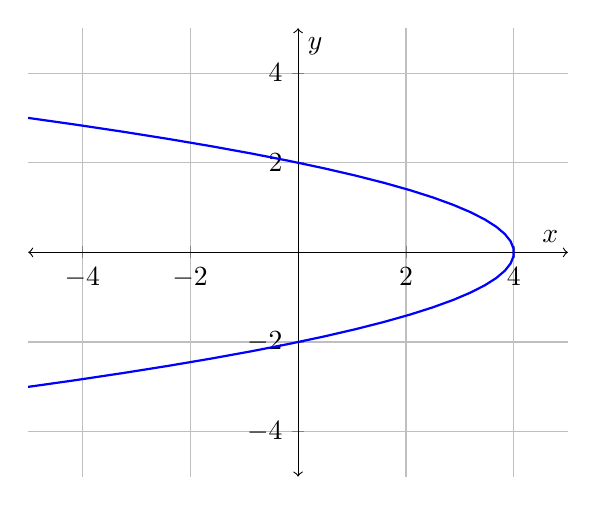
\begin{tikzpicture}
    \begin{axis}[xmin=-5,xmax=5,ymin=-5,ymax=5]
        \addplot[blue,thick,mark=none,domain=-4:4 ,samples=50] ({4-x^2},{x});
    \end{axis}
 \end{tikzpicture}
 \end{center}

 
 \begin{parts}

    \part Try parametezing the curve by setting \(x=t\) and explain what makes that approach difficult (there is not one correct answer)..
        \ifprintanswers
            \begin{solution}
                Let \(x=t\). Then 
                \[
                    t+y^2 = 4 \bif y^2 = 4-t \bif y=\pm\sqrt{4-t}\ldots
                \]
            \end{solution}
        \else
            \vfill
        \fi
    \part Now try parameterizing by setting \(y=t\).
        \ifprintanswers
            \begin{solution}
                Let \(y=t\). Then 
                \[
                    x+t^2=4 \quad\iff\quad x=4-t^2
                \]
                and we have the vector equation
                \[
                    \br(t)=\gen{4-t^2,t}
                \]
            \end{solution}
        \else
            \vfill
        \fi
    \part Verify the vector function you found satisfies \(x+y^2=4\) for any arbitrary choice of \(t\).
        \ifprintanswers
            \begin{solution}
            \begin{align*}
                x + y^2 & = 4\\
                (4-t^2)+(t^2) & = 4\\
                4 & = 4
            \end{align*}
            \end{solution}
        \else
            \vfill
        \fi
    

    \part What would you do differently for the curve \(x^2+y=4?\)
    \ifprintanswers
            \begin{solution}
                Almost nothing. The roles of \(x\) and \(y\) are exchanged in the parameterization, i.e. set \(x=t\) etc.
            \end{solution}
        \else
            \vfill
        \fi
    \end{parts}


\newpage

\question Find a vector function \(\br(t)\) that represents the curve \(x^2+16y^2=4\)
\begin{center}
 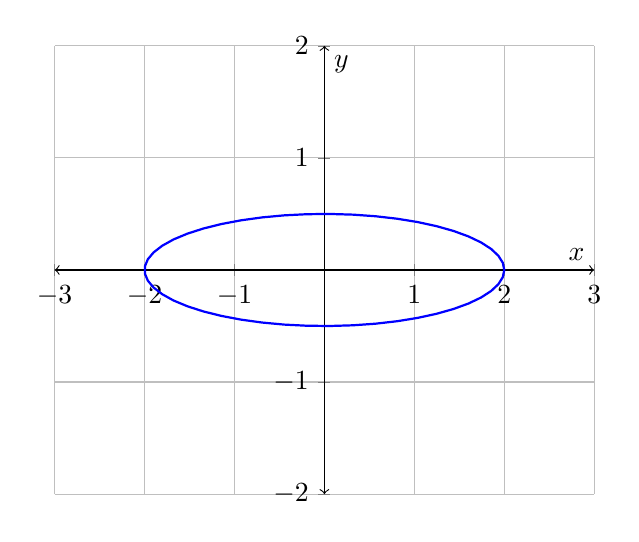
\begin{tikzpicture}
    \begin{axis}[xmin=-3,xmax=3,ymin=-2,ymax=2]
        \addplot[variable=t,blue,thick,domain=0:360 ,samples=50] ({2*cos(t)},{(1/2)*sin(t)});
    \end{axis}
 \end{tikzpicture}
 \end{center}
\begin{parts}
    \part Try parameterizing by setting \(x=t\) and then try setting \(y=t\). What makes these so difficult to work with?
    \ifprintanswers
            \begin{solution}
                If we set \(x=t\), then \(t^2+16y^2=4\) gives \(y=\pm\frac{\sqrt{4-t^2}}{4}\) which is not ideal. Setting \(y=t\) is similar.
            \end{solution}
        \else
            \vfill
        \fi

    \part Rewrite the above equation so that it has the form 
    \[
        (f(x))^2+(g(y))^2=1
    \]

    \ifprintanswers
            \begin{solution}
                Divide by 4:
                \[
                    \frac{x^2}{4}+4y^2=1 \bif \left(\frac{x}{2}\right)^2+(2y)^2=1
                \]
            \end{solution}
        \else
            \vfill
        \fi

    \part Find \(\br(t)\) by setting \(f(x)=\cos t\) and \(g(y)=\sin t\). Be sure to include the domain for \(t\).
        \ifprintanswers
            \begin{solution}
                From 
                \[
                    \frac{x}{2}=\cos(t) \quad\text{and}\quad 2y=\sin(t)
                \]
                we get the parameterization
                \[
                    \br(t) = \gen{2\cos(t),\frac{1}{2}\sin(t)}, \quad 0\le t\le 2\pi
                \]
            \end{solution}
        \else
            \vfill
        \fi

    \part What do you need to change to represent the portion of \(x^2+36y^2=4\) where \(y\ge 0\)? What about \(x> 0\)?
    \ifprintanswers
            \begin{solution}
                There are multiple correct ways to adjust this. One example: since \(y\ge 0\) corresponds to the upper half of the ellipse, we can simply restrict the domain of \(t\) to \(0\le t\le \pi\).
                For \(x>0\), we can use \(-\pi/2 < t <\pi/2\)
            \end{solution}
        \else
            \vfill
        \fi    
\end{parts}

\newpage

\subsection*{Parameterizing curves in \(\R^3\)}

\question Find a vector function that represents the curve of intersection between the two surfaces 
\[
    y=4z^2+x^2 \quad\text{and}\quad x=z^2
\]
Hint: Try \(x=t\), \(y=t\), and \(z=t\) and see which gives you something you can work with.

    \ifprintanswers
            \begin{solution}
                \begin{align*}
                    x=t:\quad & \Rightarrow ~ z=\pm \sqrt{x}\ldots\\
                    y=t:\quad & \Rightarrow ~ t=4z^2+x^2\ldots\\
                    z=t:\quad & \Rightarrow ~ x=t^2~~\Rightarrow~~y=4t^2+t^4
                \end{align*}
            
            \end{solution}
        \else
            \vfill
        \fi
\end{questions}

\end{document}

